\section{Results}\label{results}

The method presented in section \ref{implementation} was tested on several depthmaps. This section provides the results from different depthmaps of fish, and MATLAB is used for making 3D plots showing the differences from the original depthmap and the enhanced depthmap. 
In addition, simulated random particle noise was added to the depthmaps and run through the enhancement method to test how well the method performs under normal to extreme conditions.


\subsection{Algorithm Test}

The method from section \ref{implementation} was tested on several depthmap images of fish and gave very good results for many of them. During implementation it was also considered to find the largest contour from the totalfocus image instead of the depthmap, but using the totalfocus image gave a less accurate contour. 

Figure \ref{fig:algorithm_test} shows the result generated from the algorithm on four different depthmaps of the same fish.
As seen, the results looks good compared to the original images. "Holes" are filled in, particles removed and the shape of the fish from the original image is preserved. 


\begin{figure}[H]
    \centering
    \begin{subfigure}{0.49\textwidth}
        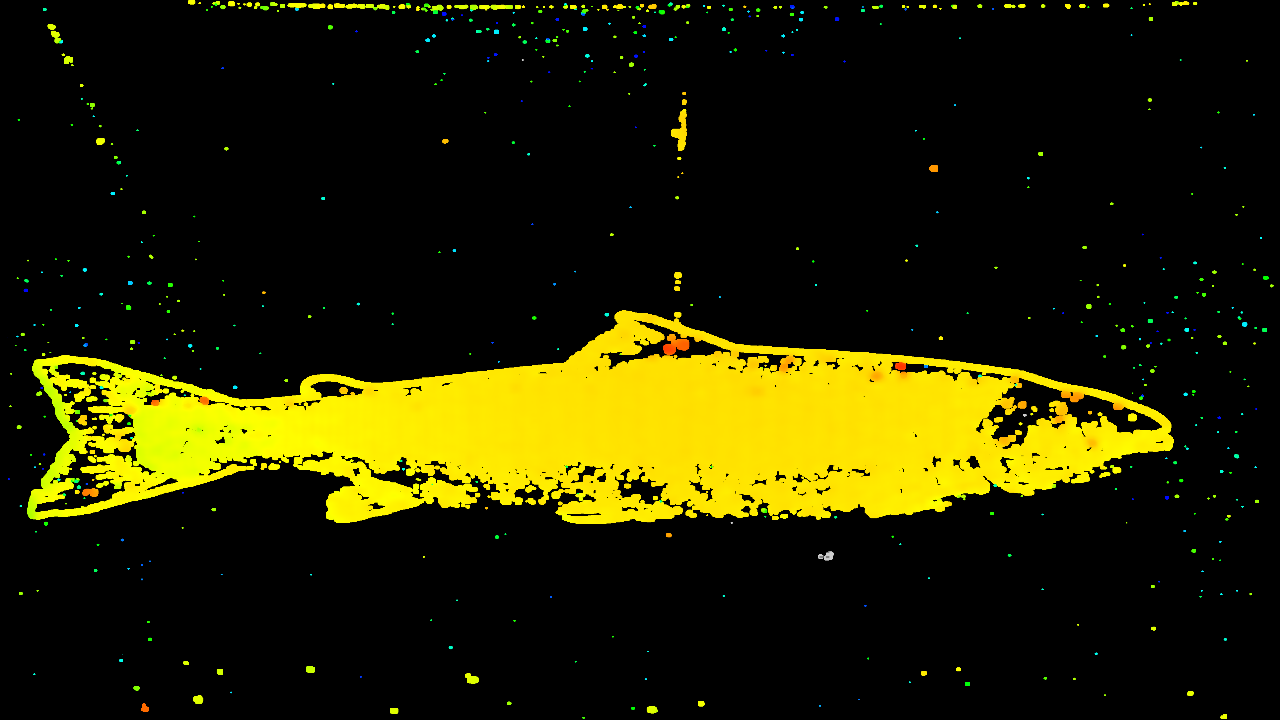
\includegraphics[width=\linewidth]{images/results/algorithm_test/original_63}
        \caption{Original Depthmap Image} 
        \label{fig:original_depthmap_63}
    \end{subfigure}\hspace*{\fill}
    \begin{subfigure}{0.49\textwidth}
        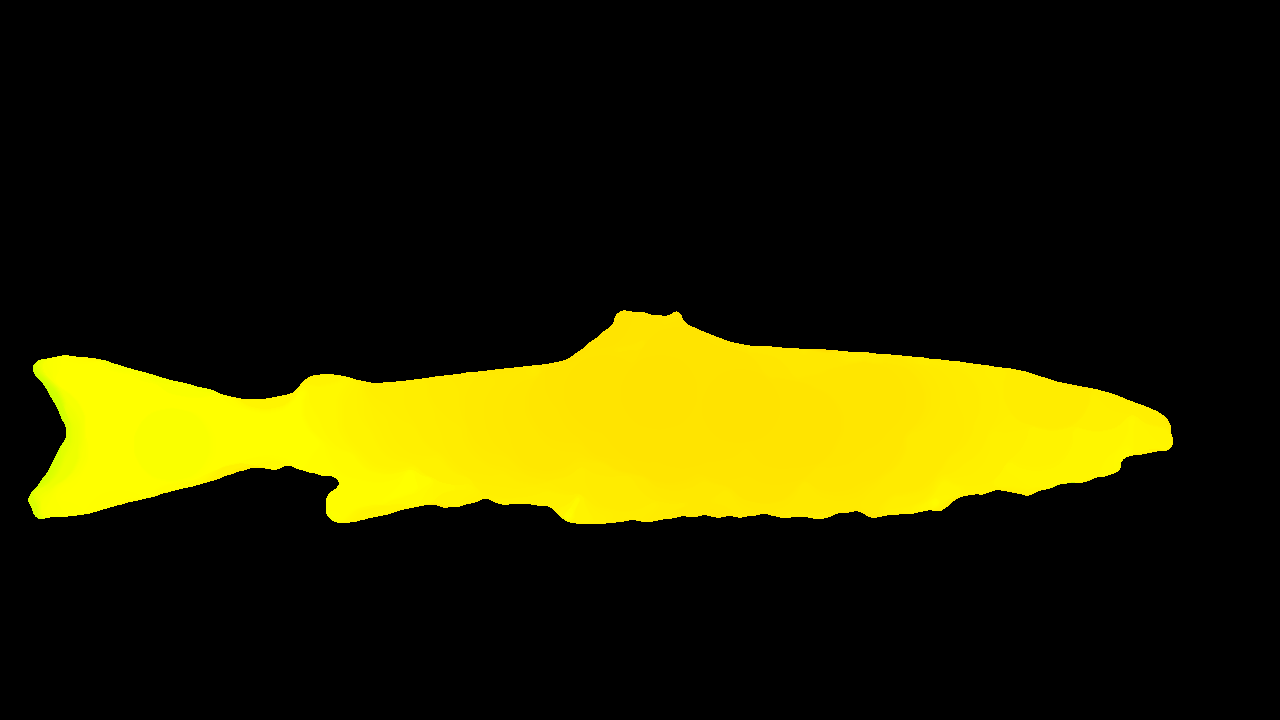
\includegraphics[width=\linewidth]{images/results/algorithm_test/median_filter_63}
        \caption{Result} 
        \label{fig:result_63}
    \end{subfigure}
    
    \medskip
    \begin{subfigure}{0.49\textwidth}
        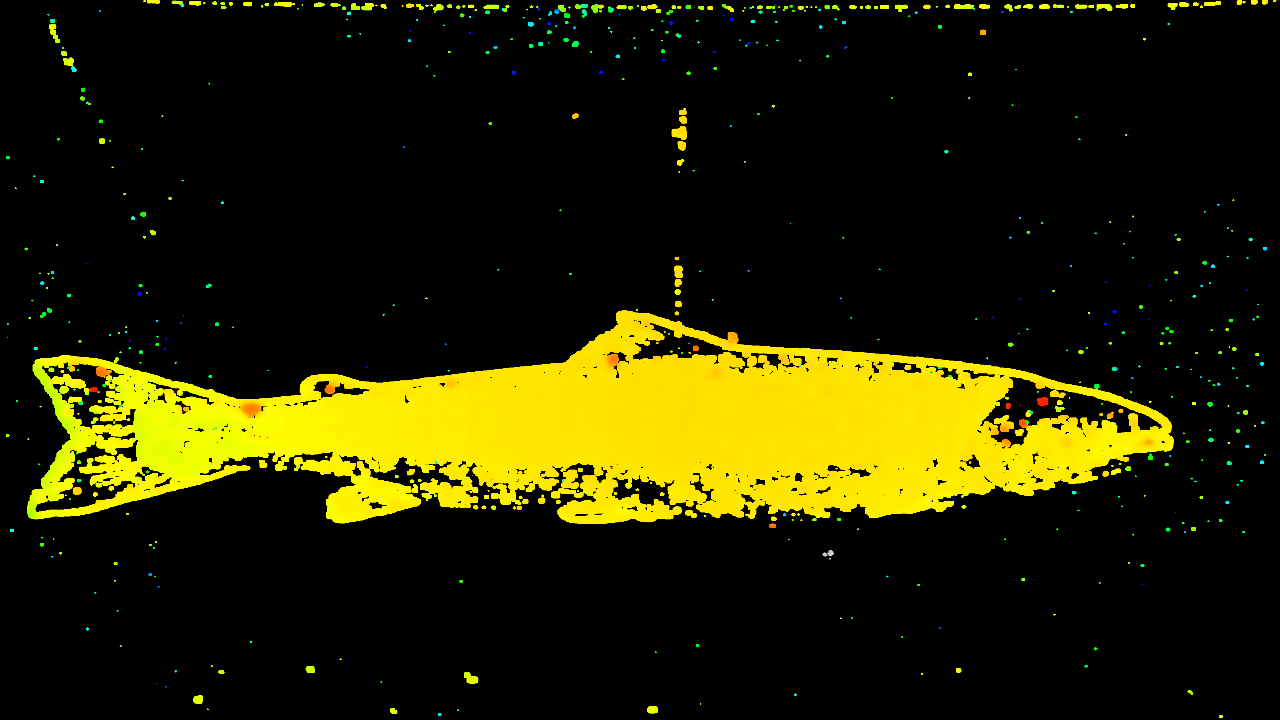
\includegraphics[width=\linewidth]{images/results/algorithm_test/original_73}
        \caption{Original Depthmap Image} 
        \label{fig:original_depthmap_73}
    \end{subfigure}\hspace*{\fill}
    \begin{subfigure}{0.49\textwidth}
        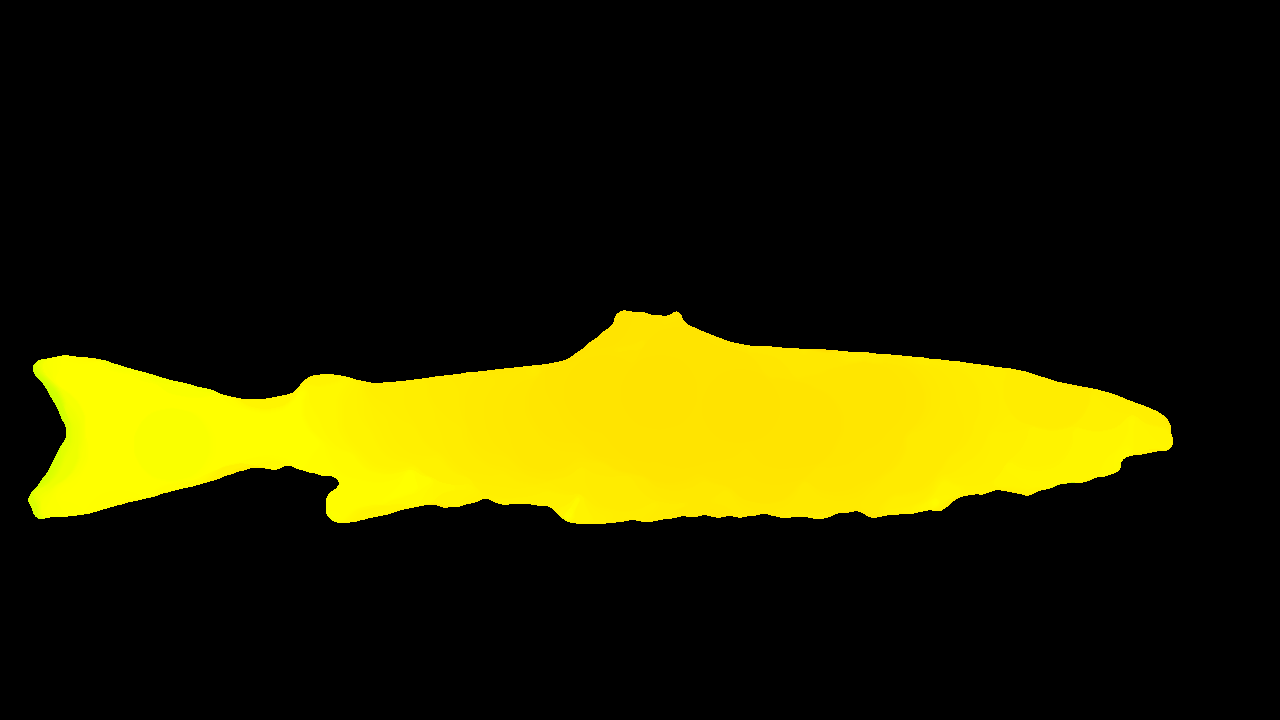
\includegraphics[width=\linewidth]{images/results/algorithm_test/median_filter_63}
        \caption{Result} 
        \label{fig:result_73}
    \end{subfigure}
    
    \medskip
    \begin{subfigure}{0.49\textwidth}
        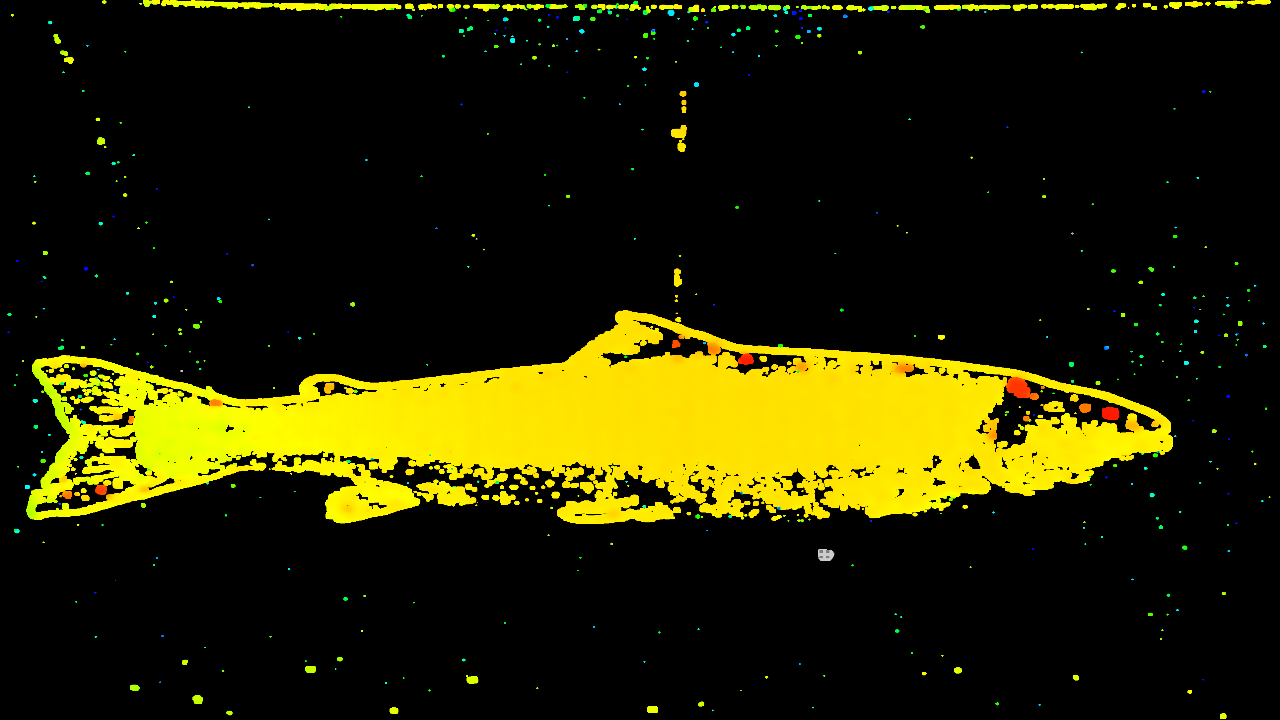
\includegraphics[width=\linewidth]{images/results/algorithm_test/original_82}
        \caption{Original Depthmap Image} 
        \label{fig:original_depthmap_82}
    \end{subfigure}\hspace*{\fill}
    \begin{subfigure}{0.49\textwidth}
        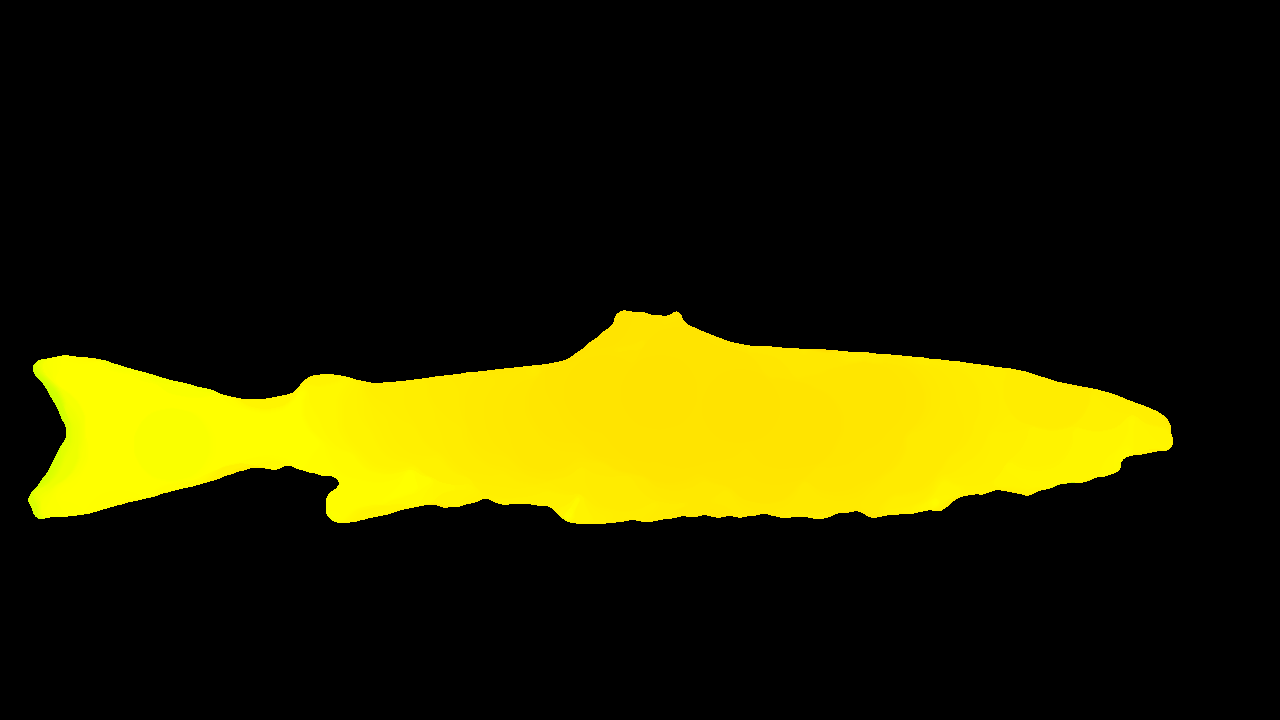
\includegraphics[width=\linewidth]{images/results/algorithm_test/median_filter_63}
        \caption{Result} 
        \label{fig:result_82}
    \end{subfigure}
    
    \medskip
    \begin{subfigure}{0.49\textwidth}
        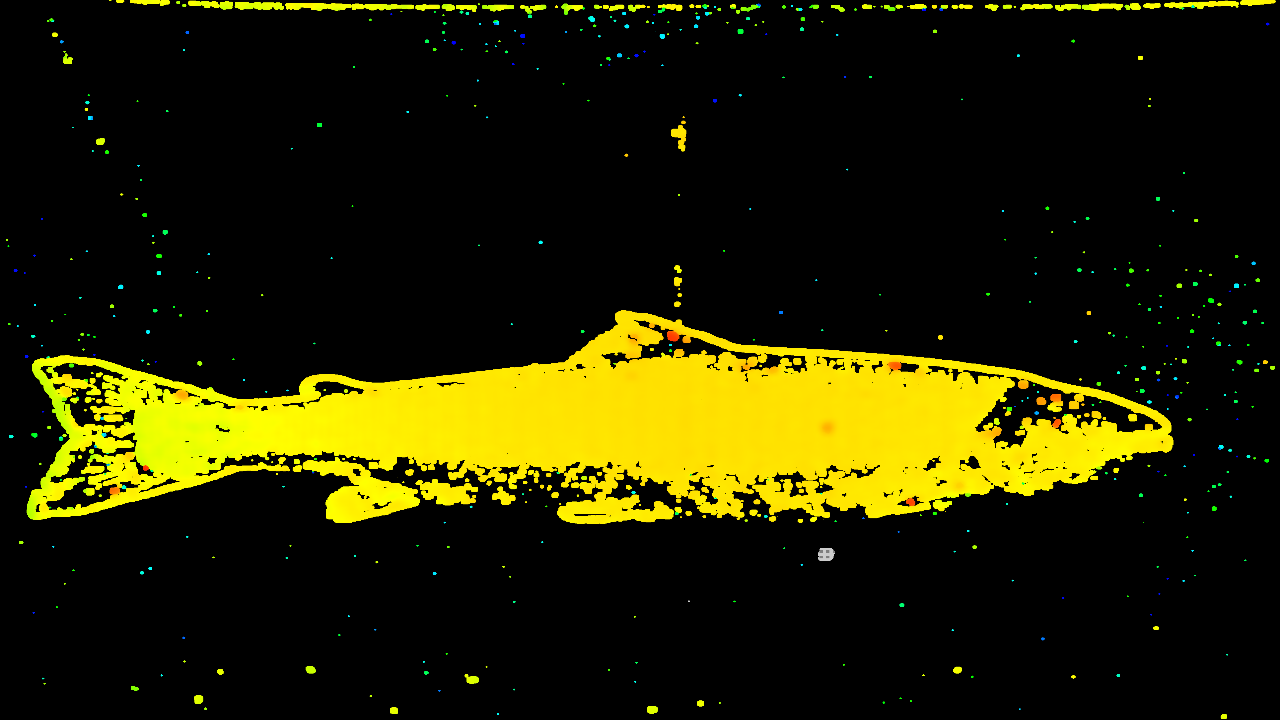
\includegraphics[width=\linewidth]{images/results/algorithm_test/original_87}
        \caption{Original Depthmap Image} 
        \label{fig:original_depthmap_87}
    \end{subfigure}\hspace*{\fill}
    \begin{subfigure}{0.49\textwidth}
        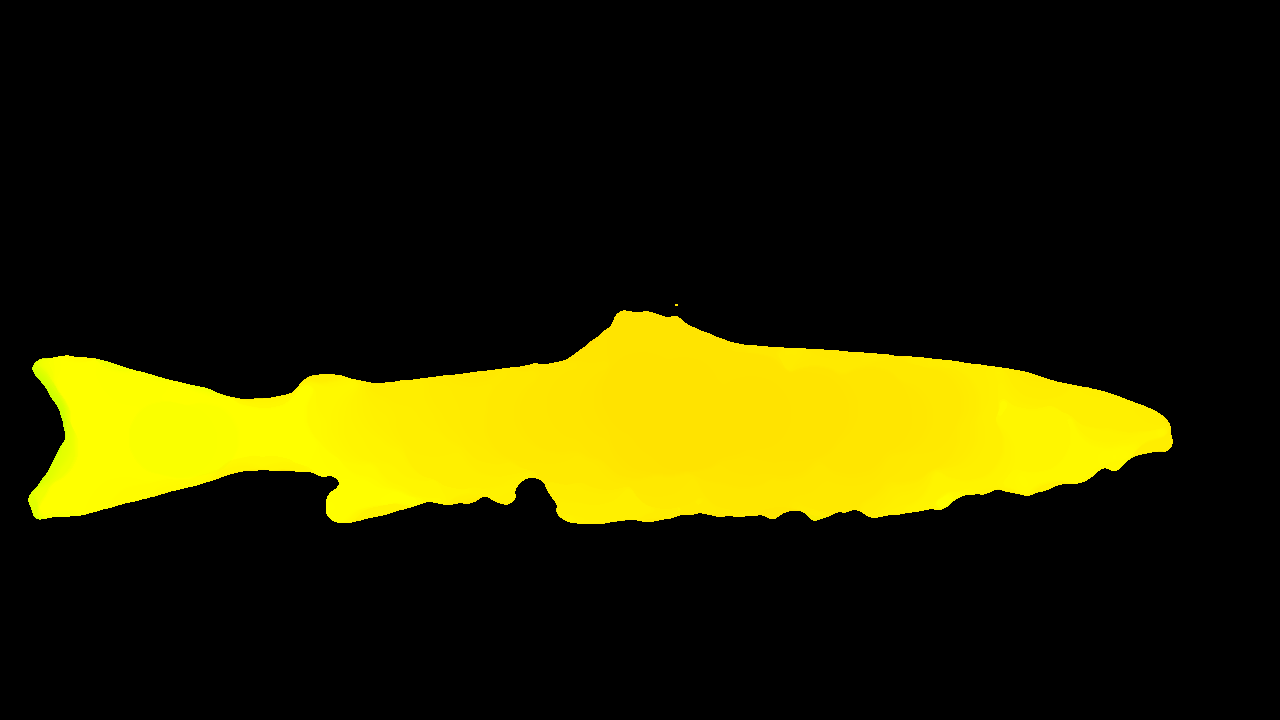
\includegraphics[width=\linewidth]{images/results/algorithm_test/median_filter_87}
        \caption{Result} 
        \label{fig:result_87}
    \end{subfigure}
    
    \caption{Algorithm Test on Different Images} 
    \label{fig:algorithm_test}
\end{figure}



%%%%%%%%%%%%%%%%%%%%%%%%%%%%%%%%%%%%%%%%%%%%%%%%%%%%%%%%%


\subsection{MATLAB 3D Plots}

To prove the results of the algorithm provided in section \ref{section:depthmap}, MATLAB was used for making a 3D plot of the fish. (See figure \ref{fig:3D_plot_63} and \ref{fig:3D_plot_87}). The MATLAB plots used the depthmaps inverted intensity values when plotting. This means that the values along the axis has no real depth value, just an intensity value between 0-255.\cite{website:mathworks_meshgrid}

From these plots it is easy to see the differences from the original depthmap to the enhanced depthmap. The totalfocus image is also put on top of the enhanced depthmap to make it even clearer that the resulting contour has nearly the same contour as the actual fish. It is also seen that most particles are removed, and the surface of the fish is evened out.

Still, some errors remain. The contour of the fish is nearly exact compared to the depthmap, but the shape of the fish in the original depthmap is not exact. Getting a more accurate shape of the fish is hard to achieve by the use of image processing, and the best way for improving this part would be through improving the imaging conditions, such as light and calibration. 
It is also seen from the 3D plots that some pixels on the fish's head and tale has got higher intensity values than it should.
This also occurs in the original image and is an error from the Raytrix computation. Luckily, this error is largest on the end of the fish's tale, and since the final goal from this implementation is volume measurement, the tale can be cut of, as it has little saying in the total volume. 

Another note about the MATLAB plot is the fact that one wrong pixel shows of really bad in the plot. So the plot can look pretty bad for an image containing just 5 bad pixel values, but a volume measurement will of course not get significantly affected.


\begin{figure}[H]
    \begin{subfigure}{0.41\textwidth}
        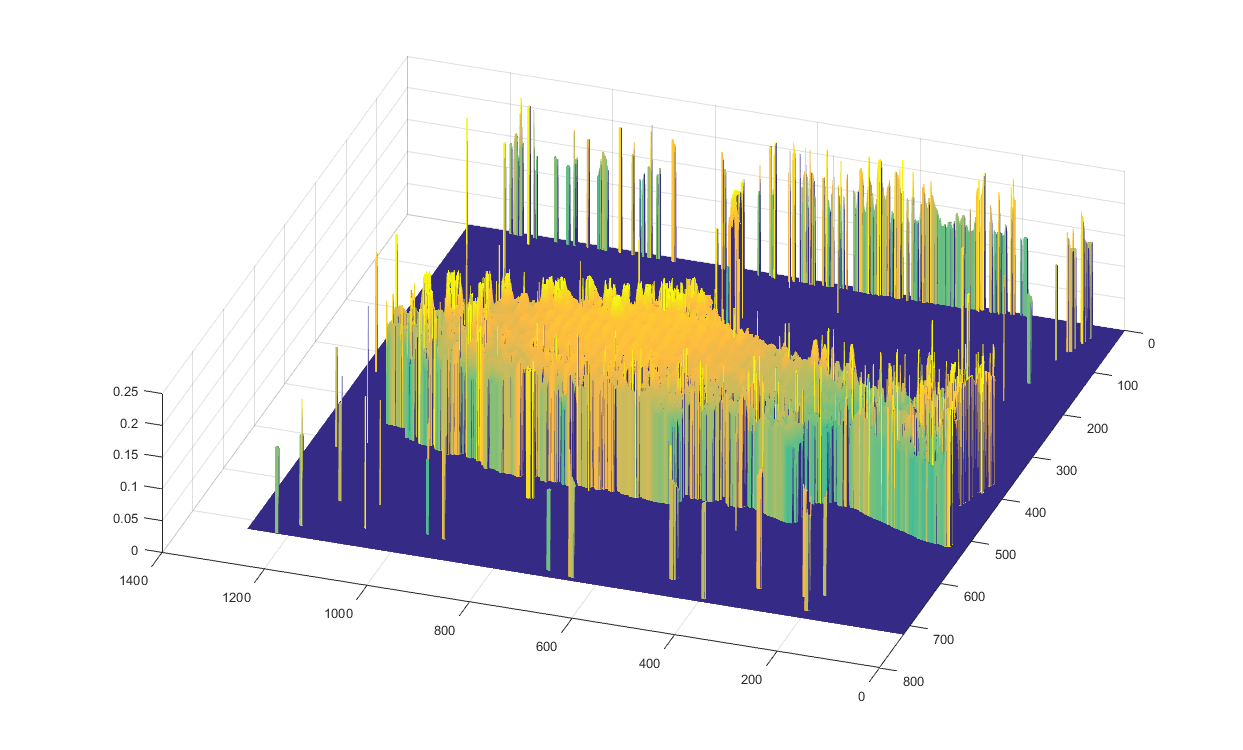
\includegraphics[width=\linewidth]{images/results/3D_plots/original_3D_63}
        \caption{Original Depthmap}
    \end{subfigure}\hspace*{\fill}
    \begin{subfigure}{0.57\textwidth}
        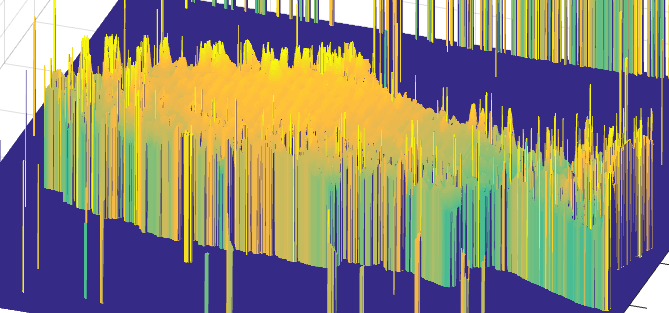
\includegraphics[width=\linewidth]{images/results/3D_plots/zoomed_original_3D_63}
        \caption{Zoomed}
    \end{subfigure}
    
    \medskip
    \begin{subfigure}{0.41\textwidth}
        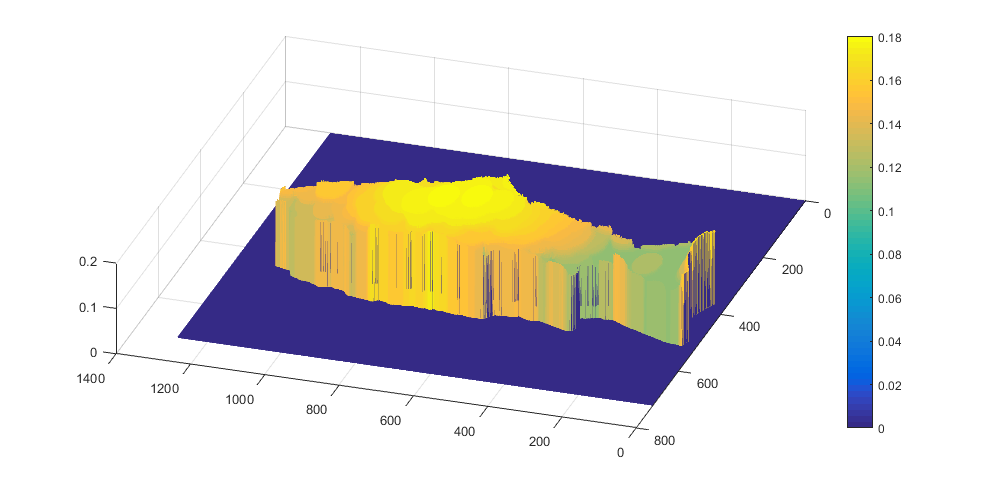
\includegraphics[width=\linewidth]{images/results/3D_plots/fixed_3D_63}
        \caption{Enhanced Depthmap}
    \end{subfigure}\hspace*{\fill}
    \begin{subfigure}{0.57\textwidth}
        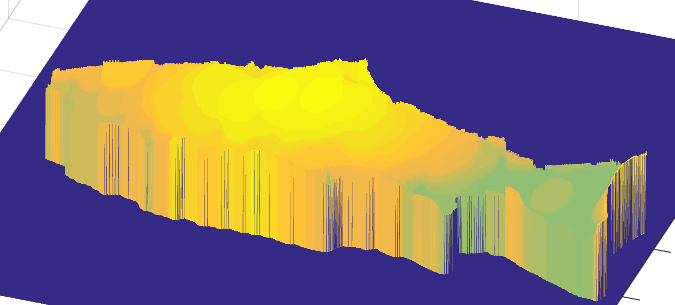
\includegraphics[width=\linewidth]{images/results/3D_plots/zoomed_fixed_3D_63}
        \caption{Zoomed}
    \end{subfigure}
    
    \medskip
    \begin{subfigure}{0.41\textwidth}
        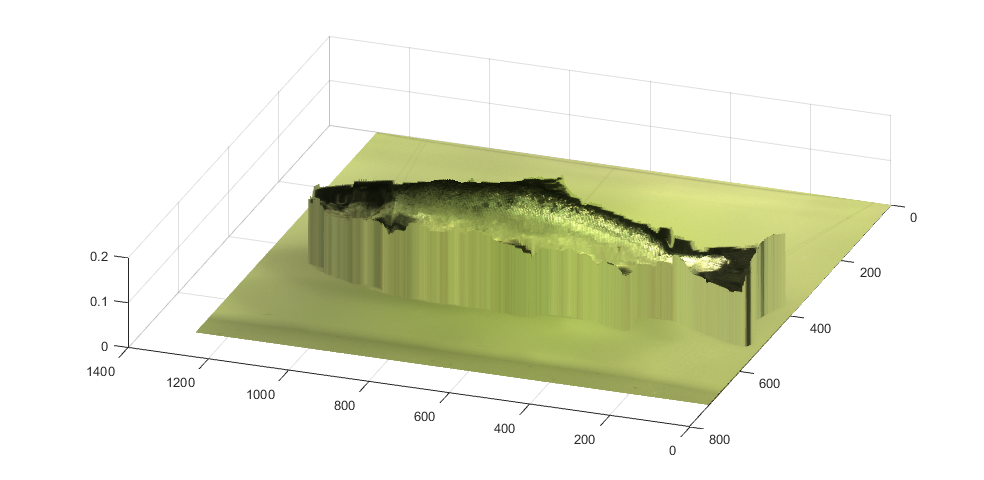
\includegraphics[width=\linewidth]{images/results/3D_plots/fixed_3D_fish_63}
        \caption{Enhanced Depthmap Overlay}
    \end{subfigure}\hspace*{\fill}
    \begin{subfigure}{0.57\textwidth}
        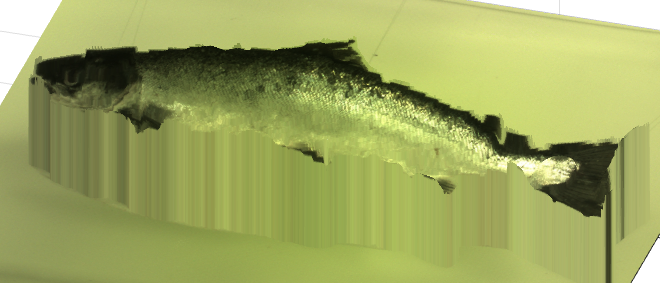
\includegraphics[width=\linewidth]{images/results/3D_plots/zoomed_fixed_3D_fish_63}
        \caption{Zoomed}
    \end{subfigure}
    
    \caption{3D Plots in MATLAB, Fish 563} 
    \label{fig:3D_plot_63}
\end{figure}


\begin{figure}[H]
    \begin{subfigure}{0.41\textwidth}
        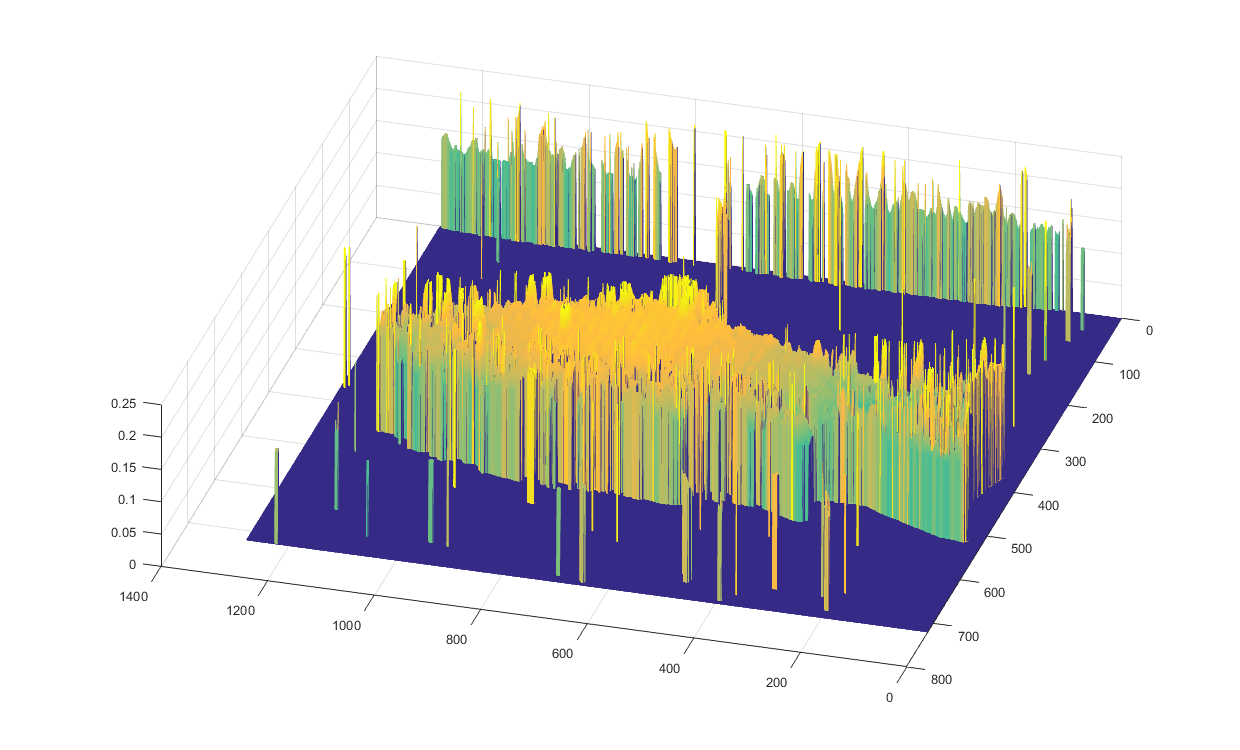
\includegraphics[width=\linewidth]{images/results/3D_plots/original_3D_87}
        \caption{Original Depthmap}
    \end{subfigure}\hspace*{\fill}
    \begin{subfigure}{0.57\textwidth}
        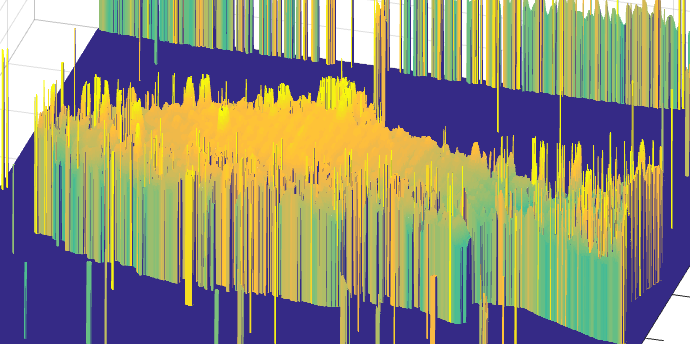
\includegraphics[width=\linewidth]{images/results/3D_plots/zoomed_original_3D_87}
        \caption{Zoomed}
    \end{subfigure}
    
    \medskip
    \begin{subfigure}{0.41\textwidth}
        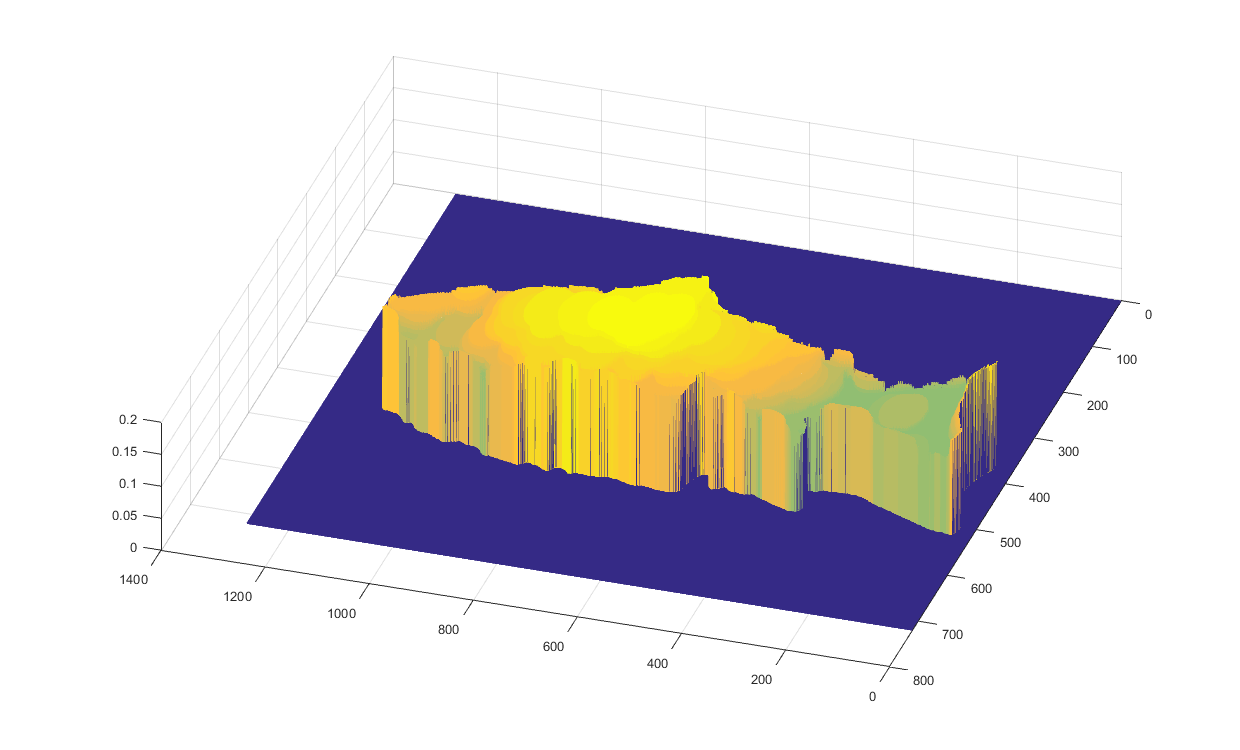
\includegraphics[width=\linewidth]{images/results/3D_plots/fixed_3D_87}
        \caption{Enhanced Depthmap}
    \end{subfigure}\hspace*{\fill}
    \begin{subfigure}{0.57\textwidth}
        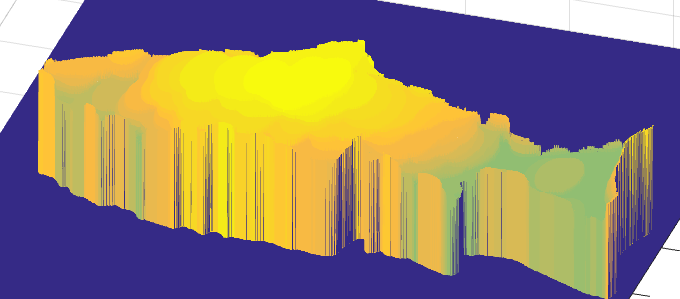
\includegraphics[width=\linewidth]{images/results/3D_plots/zoomed_fixed_3D_87}
        \caption{Zoomed}
    \end{subfigure}
    
    \medskip
    \begin{subfigure}{0.41\textwidth}
        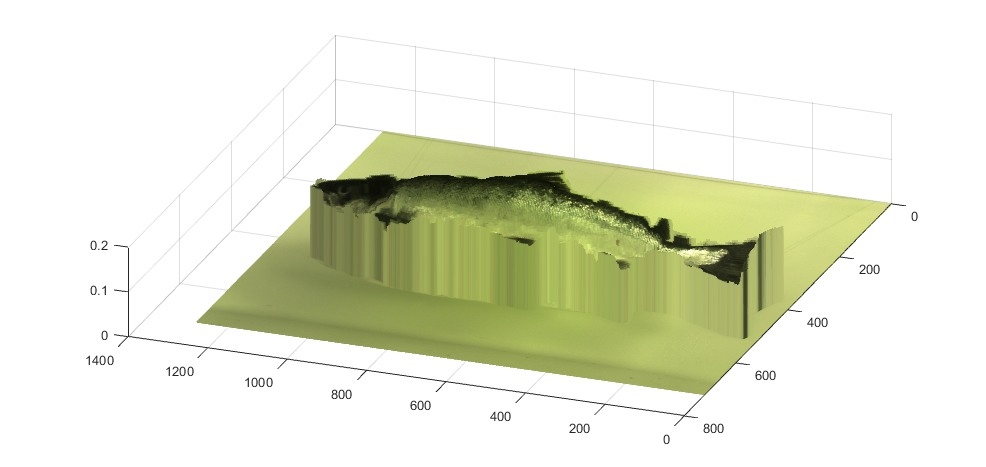
\includegraphics[width=\linewidth]{images/results/3D_plots/fixed_3D_fish_87}
        \caption{Enhanced Depthmap Overlay}
    \end{subfigure}\hspace*{\fill}
    \begin{subfigure}{0.57\textwidth}
        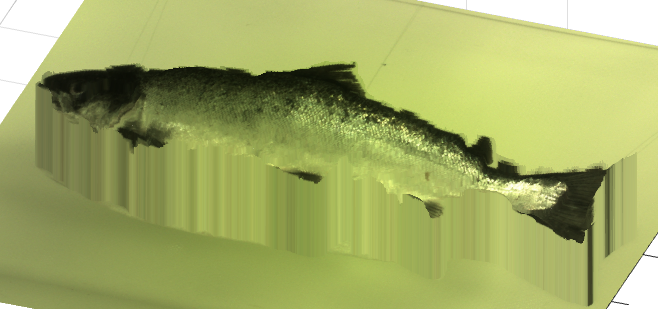
\includegraphics[width=\linewidth]{images/results/3D_plots/zoomed_fixed_3D_fish_87}
        \caption{Zoomed}
    \end{subfigure}
    
    \caption{3D Plots in MATLAB, Fish 587} 
    \label{fig:3D_plot_87}
\end{figure}
\newpage


%%%%%%%%%%%%%%%%%%%%%%%%%%%%%%%%%%%%%%%%%%%%%%%%%%%%%%%%%


\subsection{Color Data Preservation}

To ensure that the correct color data from the depthmap is not changed in the enhanced depthmap, a MATLAB plot is provided for one row of the depthmap along the fish. See figure \ref{fig:sectional} and \ref{fig:row_plot}. This plot shows the intensity values from the depthmap images, the original (red line) and the enhanced (blue line). The fish's head is to the right and its tale to the left. From the red line it is easy to see that most error on the original depthmap is found at the tail and the head, while the color data along the middle of the fish is reasonable. From figure \ref{fig:plot1} it is also seen that the correct color data is preserved and that the added data for the "holes" is within reason. It is though clear that there is still room for improvement for filling in color data at the head and tail. 
The row represented is chosen because of its bad base values in the original depthmap, so it represents one of the worst outcomes.


\begin{figure}[H]
    \centering
    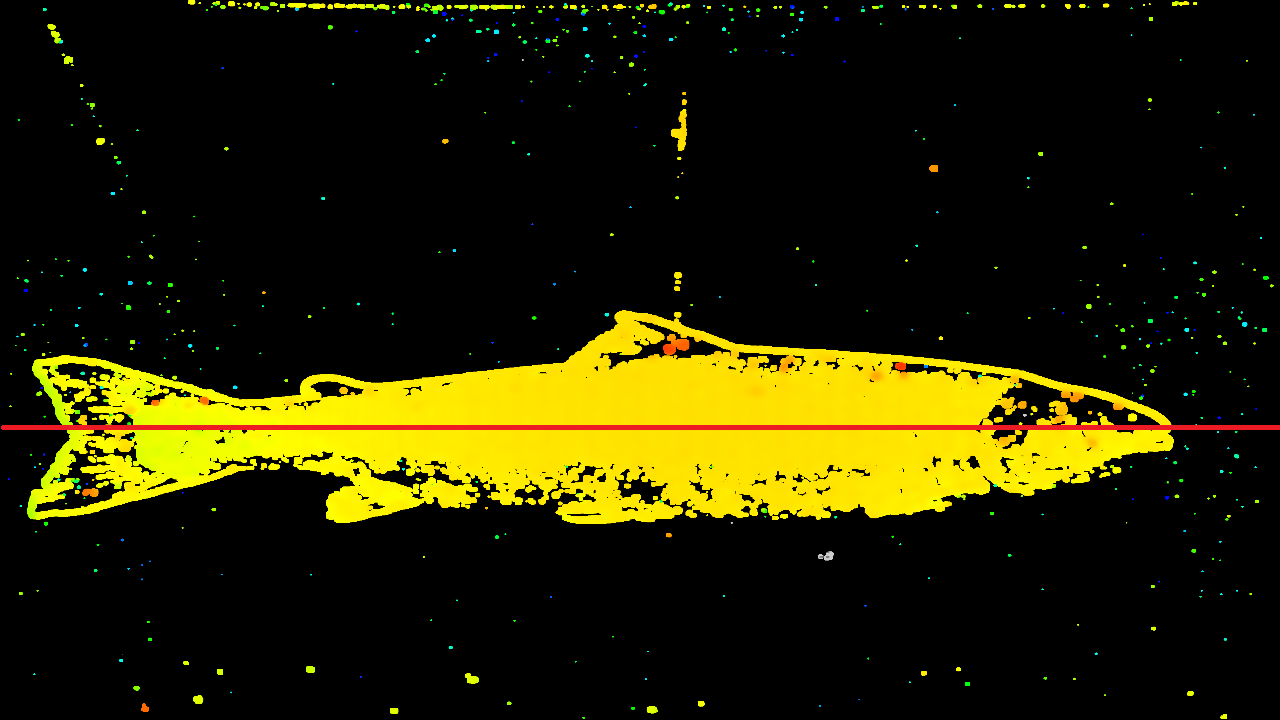
\includegraphics[width=.7\linewidth]{images/results/sectional}
    \caption{Plotted Row of Color Depth Information}
    \label{fig:sectional}
\end{figure}


\begin{figure}[H]
    \centering
    \begin{subfigure}{1\textwidth}
        \centering
        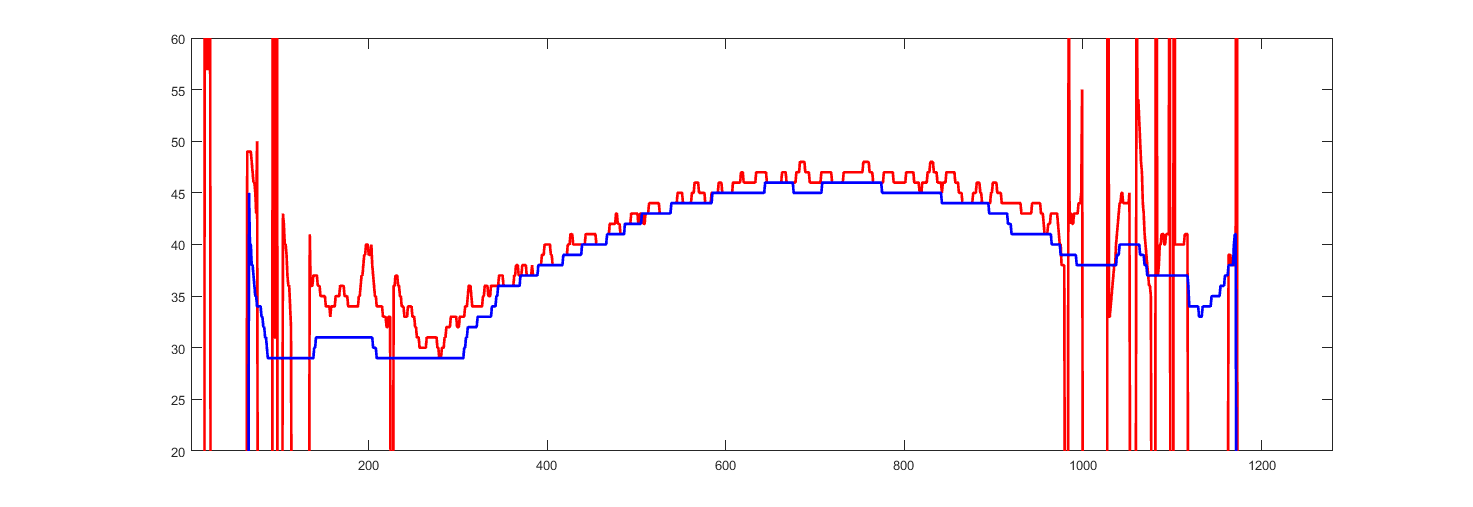
\includegraphics[width=1\linewidth]{images/results/plot_row}
        \caption{Plotted Cross Section form Depthmap} 
        \label{fig:plot1}
    \end{subfigure}\hspace*{\fill}
    
    \medskip
    \begin{subfigure}{1\textwidth}
        \centering
        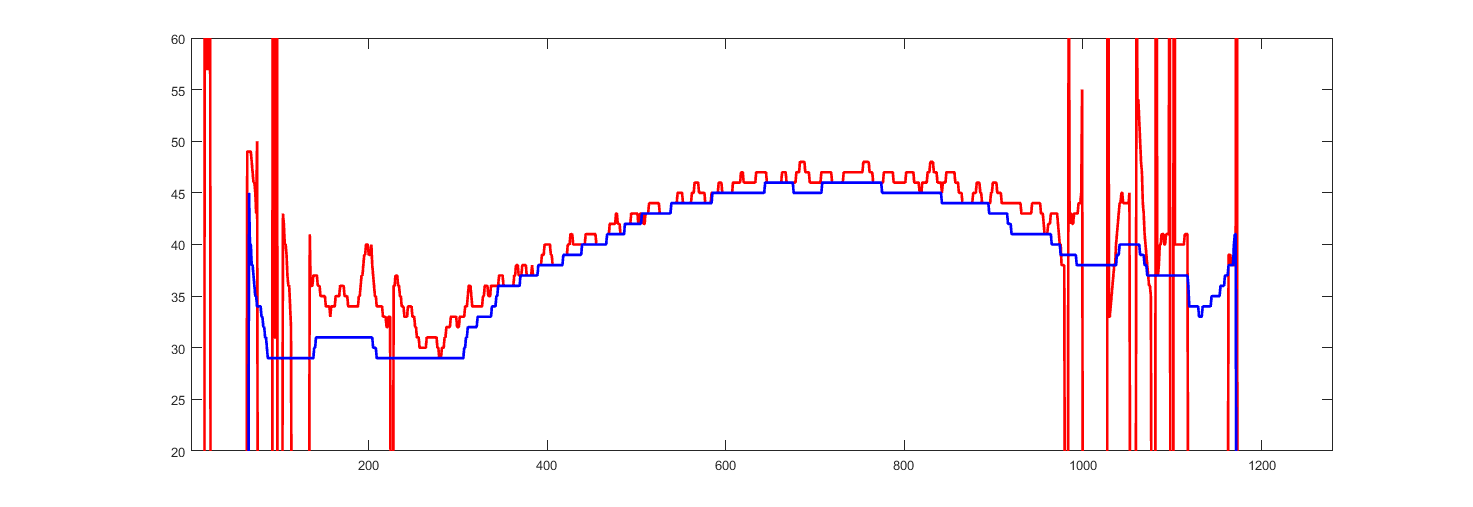
\includegraphics[width=1\linewidth]{images/results/plot_zoomed}
        \caption{Plotted Cross Section from Depthmap, Zoomed} 
        \label{fig:plot2}
    \end{subfigure}\hspace*{\fill}
    \caption{Plot of Color Depth Information}
    \label{fig:row_plot}
\end{figure}


%%%%%%%%%%%%%%%%%%%%%%%%%%%%%%%%%%%%%%%%%%%%%%%%%%%%%%%%%


\subsection{Different Levels of Particle Noise} \label{section:noise}

To make the algorithm suitable for different water conditions, simulated random particle noise was added to the depthmap. The noise added contained of random sized circles with random color placed randomly. The radius of each circle is between 1 and 6 pixels.
Noise was added from level 1 to 40, where level 1 starts with 20 particles, and each level adds 40 particles. That is, level 40 has 1,580 random particles in the image.

The algorithm had few problems up to level 20. Figure \ref{fig:noise_level_1} and figure \ref{fig:noise_level_8} shows noise level 1 and 8, respectively, and it is seen that the algorithm performs well. After level 20, small parts of the fish starts missing (figure \ref{fig:noise_level_22}), and those parts get bigger and more concentrated up to level 40. Still, the algorithm can sometimes get decent results, an example is at noise level 32 (figure \ref{fig:noise_level_32}). Level 40 is almost covered with particles, and this would most likely never be a real issue, but the results are still surprisingly good.

If the algorithm is to be used in conditions containing more particles than level 20, it is reasonable to believe that some more processing and tuning could give sufficient results also then. The case would most likely be to fill in the missing parts even more, and perhaps calculate the largest contour from the totalfocus image instead of the depthmap. This is though such extreme particle conditions that it is not reasonable to believe that such conditions will occur for the given problem.


\begin{figure}[H]
    \centering
    \begin{subfigure}{0.5\textwidth}
        \centering
        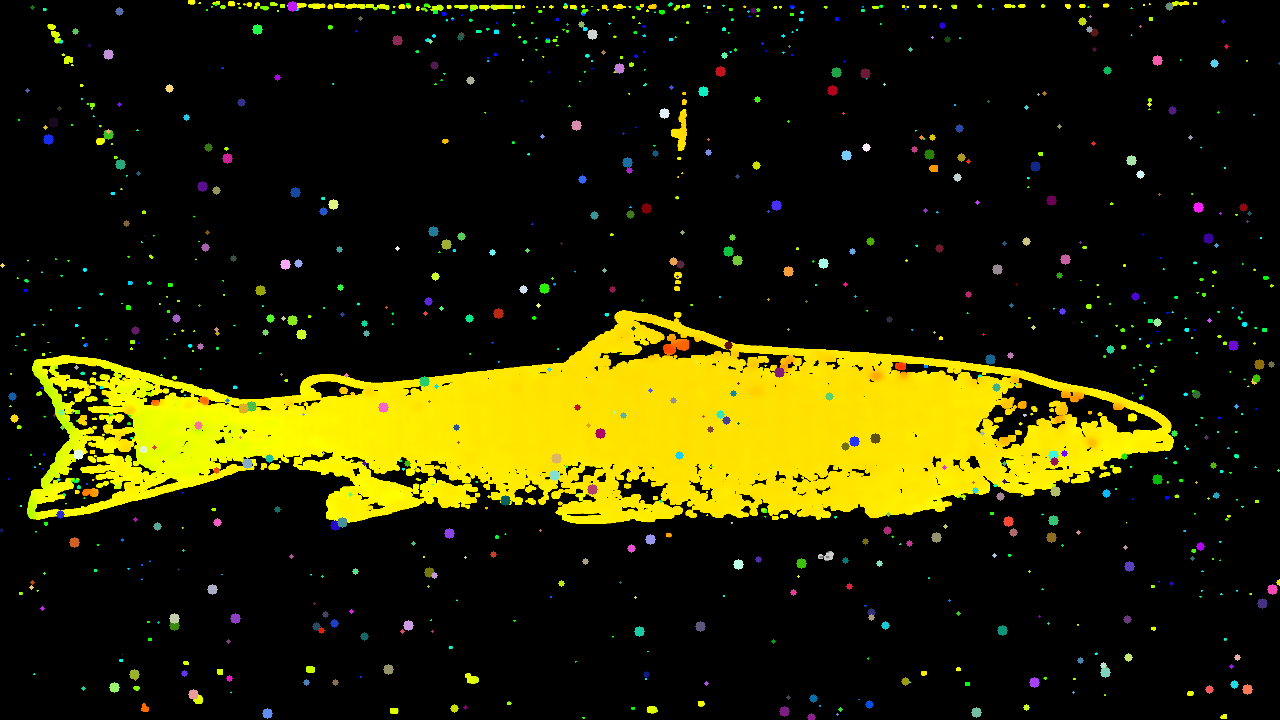
\includegraphics[width=.95\linewidth]{images/results/noise/noise63_1}
        \caption{Depthmap Image with Noise Level 1} 
        \label{fig:image_noise_level_1}
    \end{subfigure}%
    \begin{subfigure}{0.5\textwidth}
        \centering
        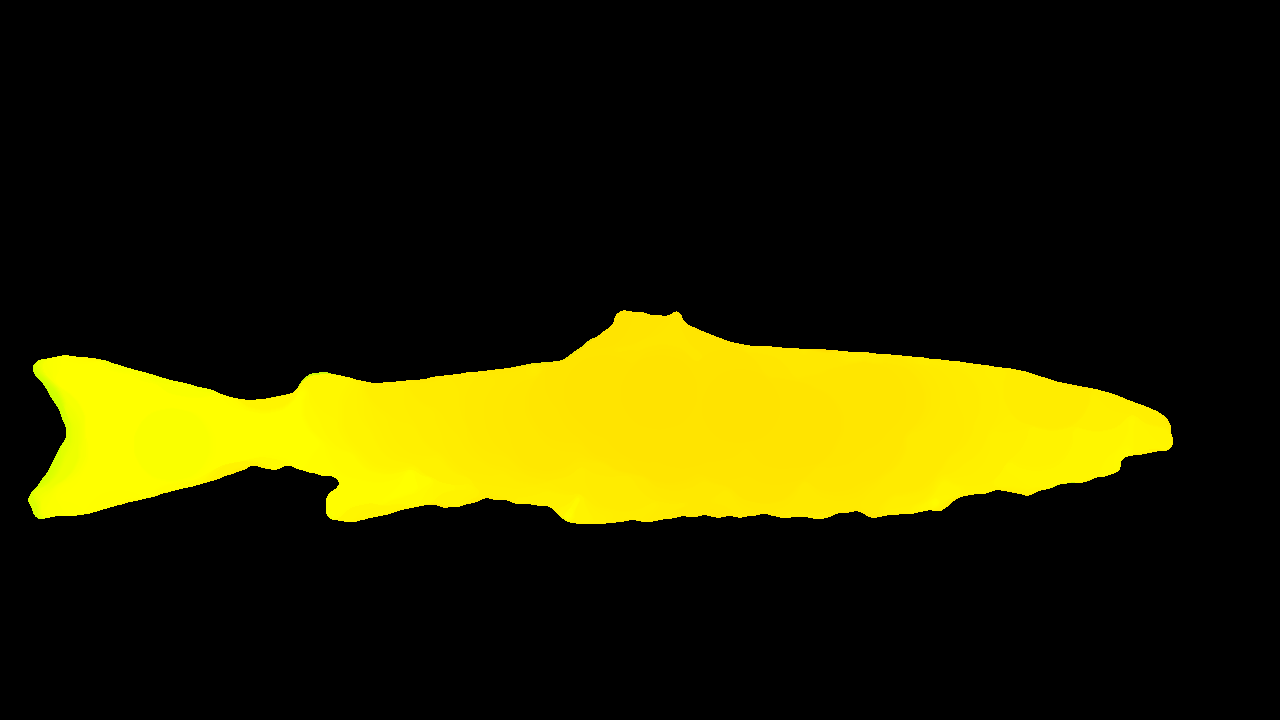
\includegraphics[width=.95\linewidth]{images/results/noise/filternoise63_1}
        \caption{Resulting Depthmap} 
        \label{fig:filter_noise_level_1}
    \end{subfigure}
    \caption{Depthmap Image and Result for Noise Level 1}
    \label{fig:noise_level_1}
\end{figure}

\begin{figure}[H]
    \centering
    \begin{subfigure}{0.5\textwidth}
        \centering
        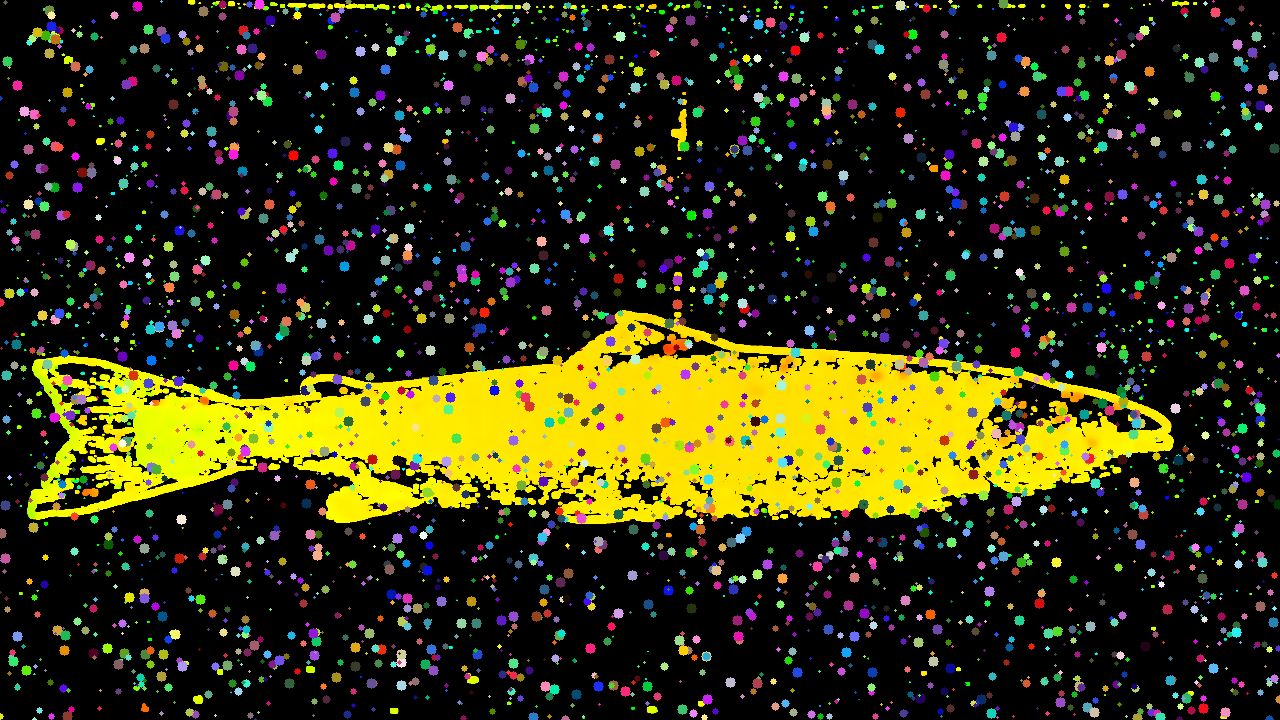
\includegraphics[width=.95\linewidth]{images/results/noise/noise63_8}
        \caption{Depthmap Image with Noise Level 8} 
        \label{fig:image_noise_level_8}
    \end{subfigure}%
    \begin{subfigure}{0.5\textwidth}
        \centering
        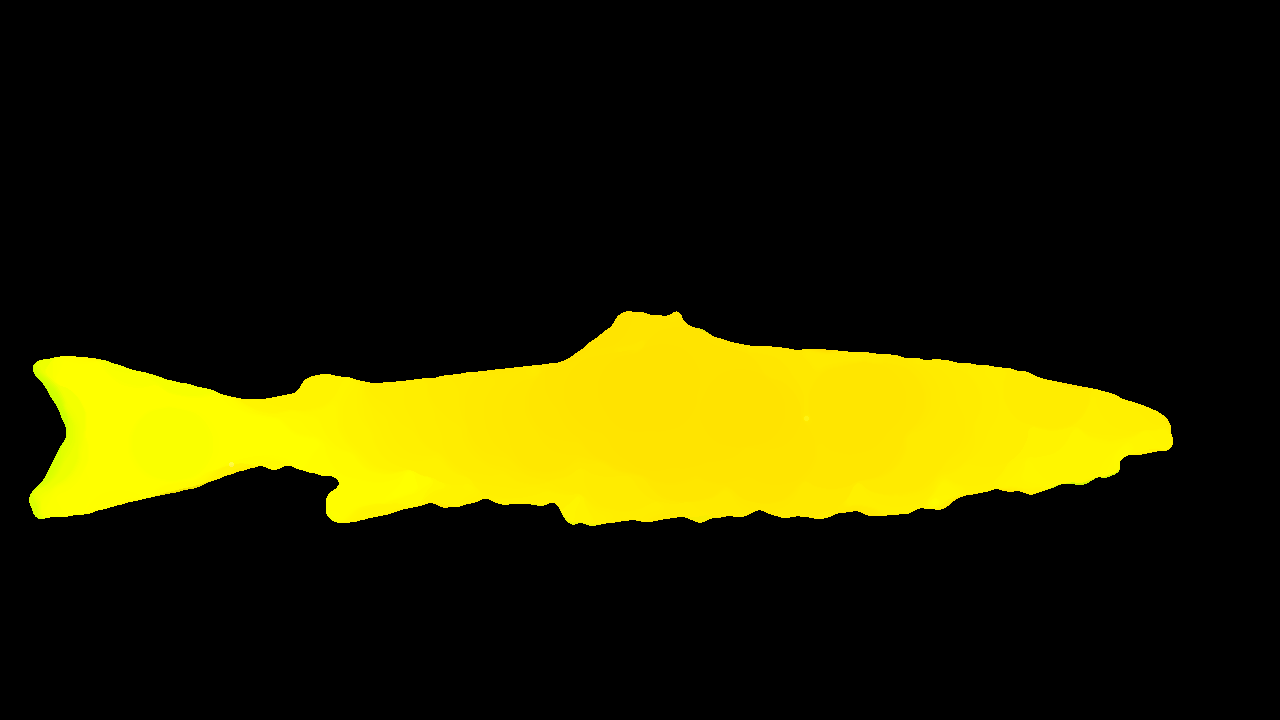
\includegraphics[width=.95\linewidth]{images/results/noise/filternoise63_8}
        \caption{Resulting Depthmap} 
        \label{fig:filter_noise_level_8}
    \end{subfigure}
    \caption{Depthmap Image and Result for Noise Level 8}
    \label{fig:noise_level_8}
\end{figure}

\begin{figure}[H]
    \centering
    \begin{subfigure}{0.5\textwidth}
        \centering
        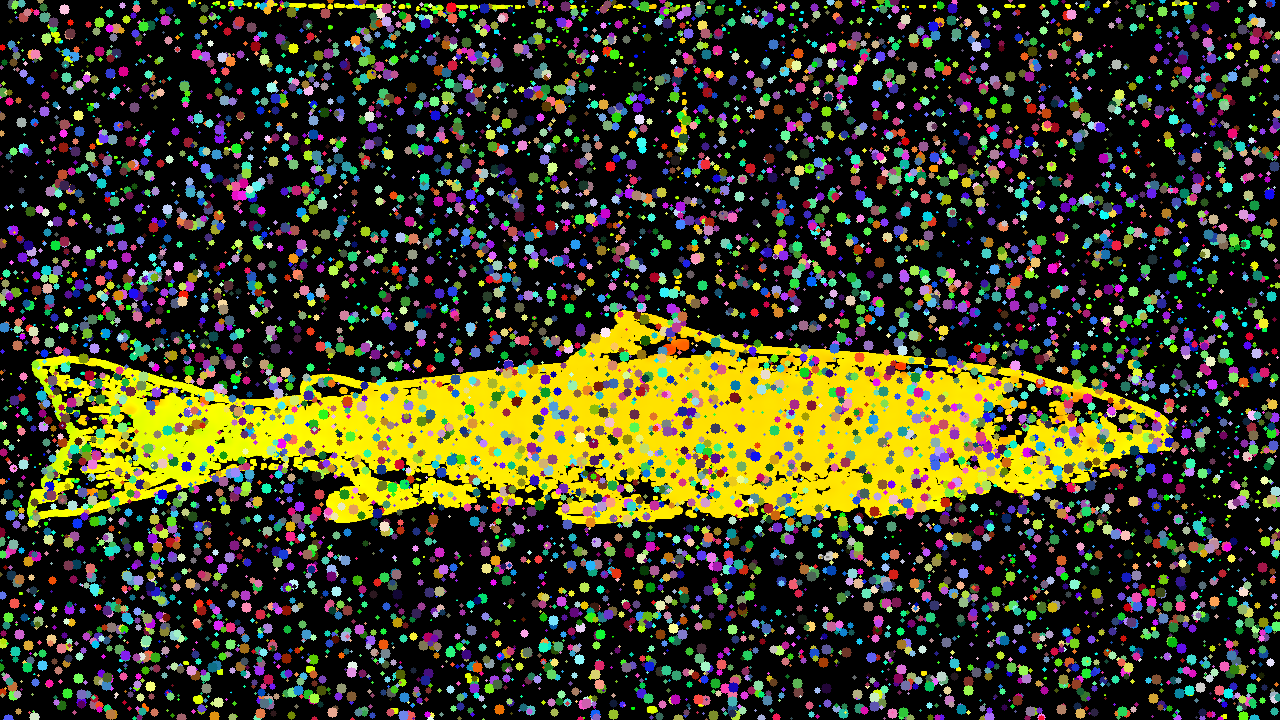
\includegraphics[width=.95\linewidth]{images/results/noise/noise63_22}
        \caption{Depthmap Image with Noise Level 22} 
        \label{fig:image_noise_level_22}
    \end{subfigure}%
    \begin{subfigure}{0.5\textwidth}
        \centering
        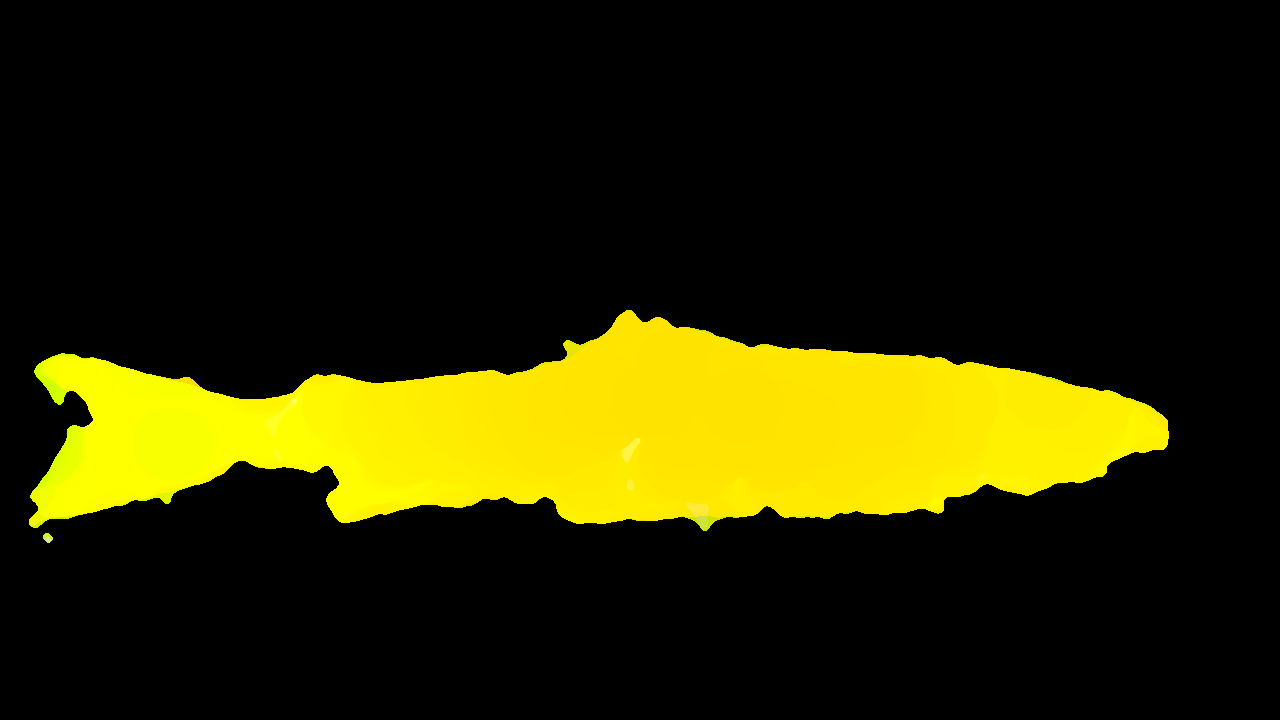
\includegraphics[width=.95\linewidth]{images/results/noise/filternoise63_22}
        \caption{Resulting Depthmap} 
        \label{fig:filter_noise_level_22}
    \end{subfigure}
    \caption{Depthmap Image and Result for Noise Level 22}
    \label{fig:noise_level_22}
\end{figure}

\begin{figure}[H]
    \centering
    \begin{subfigure}{0.5\textwidth}
        \centering
        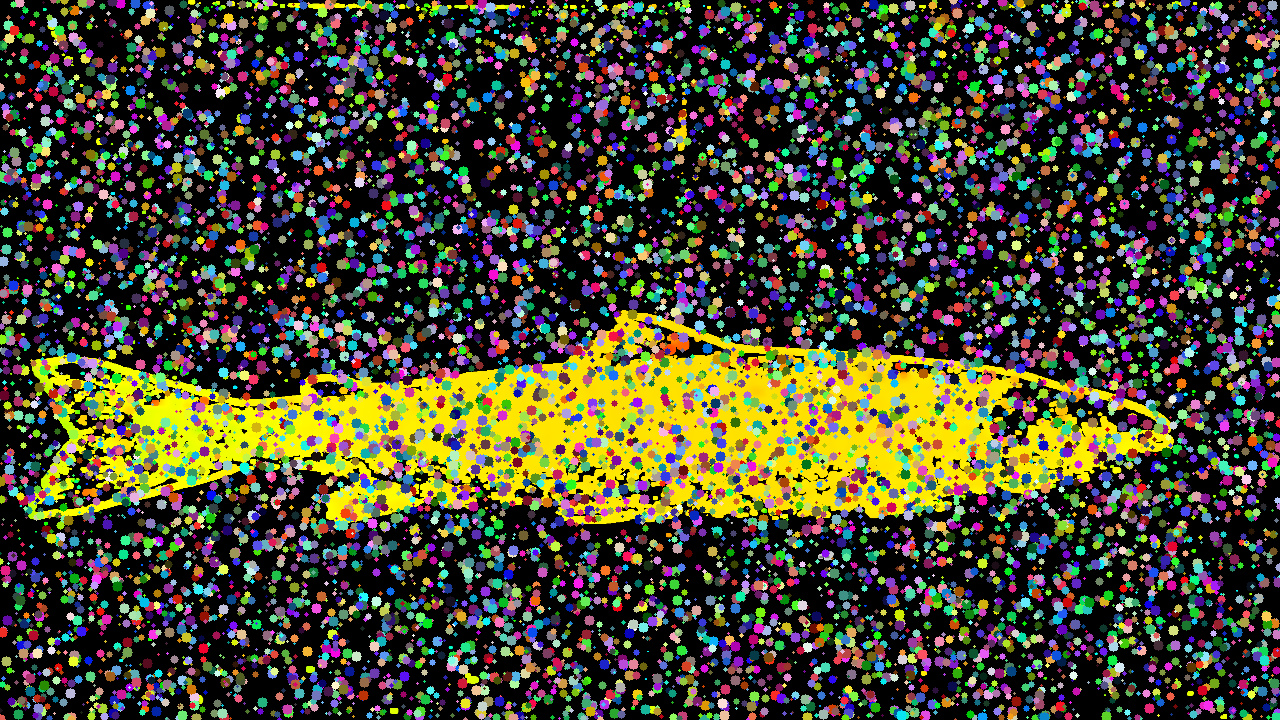
\includegraphics[width=.95\linewidth]{images/results/noise/noise63_32}
        \caption{Depthmap Image with Noise Level 32} 
        \label{fig:image_noise_level_32}
    \end{subfigure}%
    \begin{subfigure}{0.5\textwidth}
        \centering
        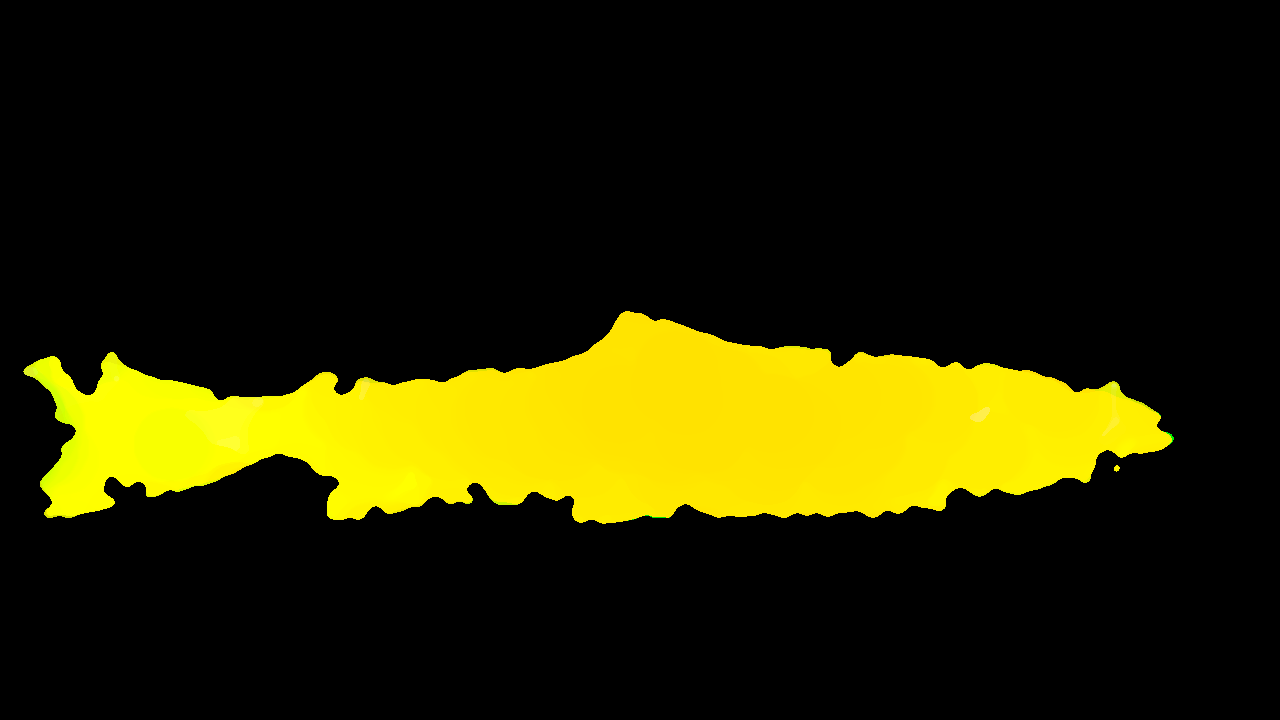
\includegraphics[width=.95\linewidth]{images/results/noise/filternoise63_32}
        \caption{Resulting Depthmap} 
        \label{fig:filter_noise_level_32}
    \end{subfigure}
    \caption{Depthmap Image and Result for Noise Level 32}
    \label{fig:noise_level_32}
\end{figure}

\begin{figure}[H]
    \centering
    \begin{subfigure}{0.5\textwidth}
        \centering
        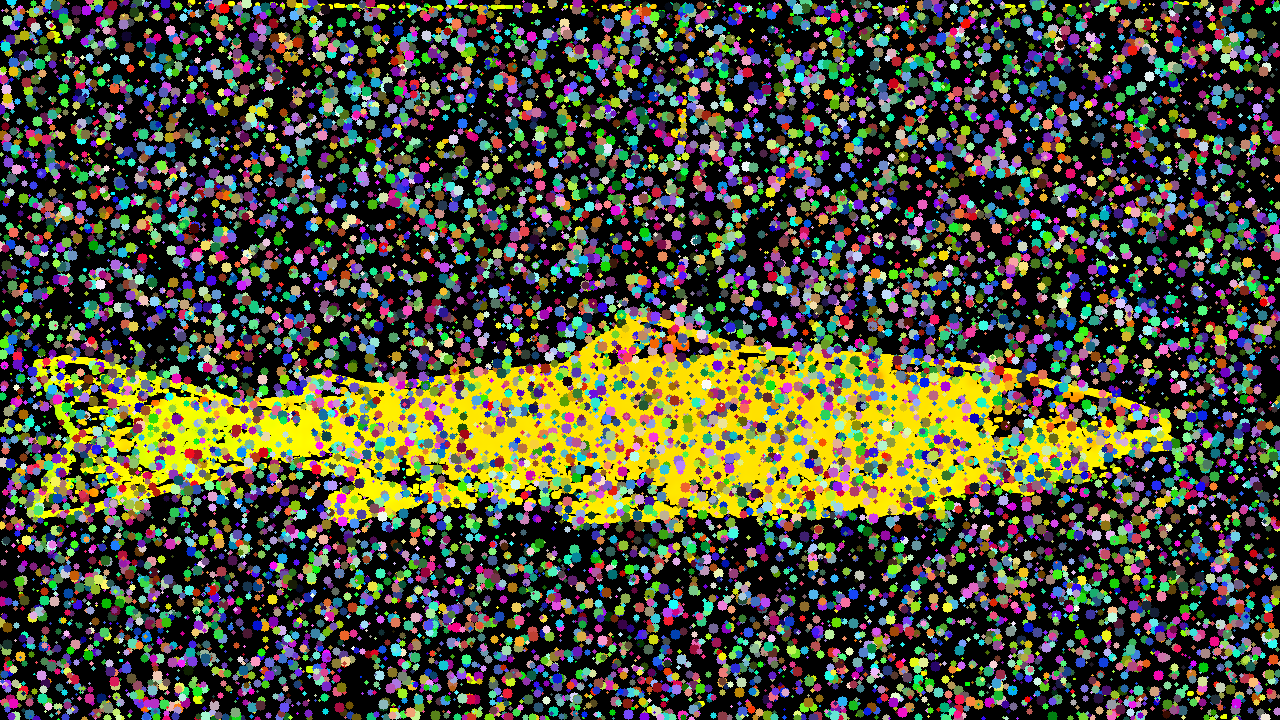
\includegraphics[width=.95\linewidth]{images/results/noise/noise63_40}
        \caption{Depthmap Image with Noise Level 40} 
        \label{fig:image_noise_level_40}
    \end{subfigure}%
    \begin{subfigure}{0.5\textwidth}
        \centering
        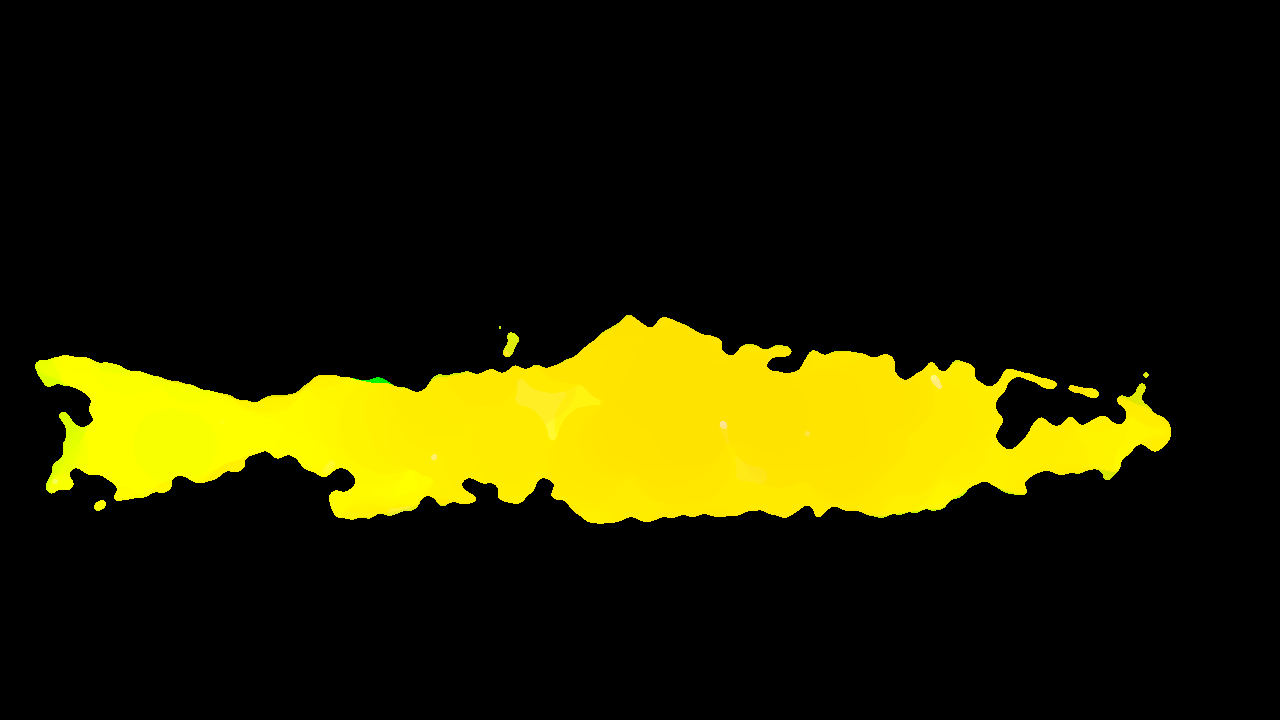
\includegraphics[width=.95\linewidth]{images/results/noise/filternoise63_40}
        \caption{Resulting Depthmap} 
        \label{fig:filter_noise_level_40}
    \end{subfigure}
    \caption{Depthmap Image and Result for Noise Level 40}
    \label{fig:noise_level_40}
\end{figure}

